\documentclass[conference]{IEEEtran}
\IEEEoverridecommandlockouts
% The preceding line is only needed to identify funding in the first footnote. If that is unneeded, please comment it out.
\usepackage{cite}
\usepackage{url}
\usepackage{amsmath,amssymb,amsfonts}
\usepackage{algorithmic}
\usepackage{graphicx}
\usepackage{textcomp}
\usepackage{xcolor}
\usepackage{footmisc}
\usepackage{tikz}

\def\BibTeX{{\rm B\kern-.05em{\sc i\kern-.025em b}\kern-.08em
    T\kern-.1667em\lower.7ex\hbox{E}\kern-.125emX}}
\begin{document}

\title{Swarm driving with Deep Learning\\
}

\author{\IEEEauthorblockN{ Luca Brodo}
\IEEEauthorblockA{\textit{Hochschule Hamm-Lippstadt)} \\
\textit{Deep Learning}\\
Lippstadt, Germany \\
luca.brodo@stud.hshl.de}

}

\maketitle

\begin{abstract}
Machine learning has completely changed what we deemed as possible and impossible. With the new doors opened in communication technologies and the advancements in deep learning, the field of swarm driving has been revolutionized. We are now able to apply swarm driving to real world application to increase safety and security, while at the same time saving money and resources. 
In this paper, we will explore what swarm driving is, what it will be in the future and how the introduction of deep learning techniques has augmented the possibilities this field has to offer making it a perfect candidate to solve some of the most complex and safety critical problems.
\end{abstract}

\begin{IEEEkeywords}
Deep Learning, Deep Reinforcement Learning, Robot Swarms, Q-Function
\end{IEEEkeywords}

\section{Motivation}
In recent years there has been an unprecedented evolution in communication technologies, introducing engineers to new horizons, which a couple of decades ago were not even imaginable. These advancements brought us a new field, namely the Internet of Things, and now every device has the possibilities to communicate with one another, hence augmenting exponentially their possibilities, since they are not limited by their on-board resources anymore. In other words, now even the smallest, less powerful device can now fulfill requirements which would have normally required a lot of memory and computational power. \\
Being able to communicate with others in a fast and reliable way, in addition to what it has already been said, allows to create situations where devices can cooperate with others to reach a common goal.\\ Cooperation has been proven in nature to exceed the capabilities of one individual and there is a plethora of examples that prove it \cite{guided}. The most shining example of teamwork in the animal kingdom are bees. A hive of honey bees consists of almost 60,000 different bees, each one having a very specific job and they contribute to the overall success of the hive the same amount\cite{MAAREC}. \\
Cooperation, however, does not exclusively bring benefits to complex tasks, it even allows individuals to solve rather simple tasks more efficiently as well. As a matter of fact, ants benefit from cooperation by transporting in groups a weight, which would otherwise be impossible to lift by a single ant. \\
What complex and non-complex situations have in common is that each individual has at its own disposal only its basic and limited sensing of the environment and could benefit from the help of the others. \cite{guided} \\
From these biological processes the field of robotic has been trying to take inspiration in order to solve very complex tasks in the real world with the use of rather simple agents. In most cases, those agents have very basic movement and communication capabilities and are only able to sense parts of the environment, yet, by cooperating, they are able to solve delicate real-time tasks in a fast and reliably way. What this translates to is systems which can solve very complex tasks with a relatively low cost of production, since they do not require expensive resources or cutting-edge technologies to operate. As M.H{\"u}ttenrauch et al. pointed out in \cite{guided}, usually to implement such cooperative systems a common approach is to extract rules from the environment. Such approach, however, if done manually, is not only tedious, but can also become in some case so complex that some tasks become unsolvable. The use of Deep Learning can obviate to this problem and at the same time augment the possibilities of the system, making it more flexible to changes and therefore scalable as well. \\Deep Learning can bring a lot of benefits, however there are nuances which should be known and techniques like Neural Network can be fiddly at times. In this paper, we will explore the use of Deep Learning techniques in swarm systems and how they can be used to create fast, efficient, reliable systems to tackle very complex problems. In order to achieve this, in the first section, we will introduce what swarm systems are and where they are applied. Subsequently, in the second and third section, we will introduce deep learning and we will define the difference between Deep Learning and Deep Reinforcement Learning. In the last section we will discuss the application Deep Learning in swarm systems with some proposed solutions. Finally, we will discuss an implementation of said techniques in a simulation of a swarm system. 
\section{Swarm robotics}\label{sec:swarm}
\textit{Swarm robotics}, as the name implies, is a branch of robotics which deals with the coordination of multiple, usually simple, robots in order to achieve a common goal, creating structures and behaviors inspired by the ones observed in nature\cite{cheraghi_past_2021}.
Swarm Robotics refers to the application of swarm principles to robotics, while \textit{Swarm intelligence} indicates to the general set of algorithms which make swarm robotics possible. \\
Beni in \cite{10.1007/978-3-540-30552-1_1} delineates various properties that swarms of robots must to replicate the idea of natural swarming efficiently. \\

Amongst all of the properties, the more important ones are:
\begin{description}
  \item[\textbf{Flexibility}] \hfill\\ Usually, in order to achieve the proposed goals, robots in a swarm need to solve a variety of tasks, therefore the system needs to be flexible. Robots should be able to find solutions for each task by working together and be able to act simultaneously and change their role according to the environment
  \item[\textbf{Scalability}] \hfill \\ The system must be able to work independently from the number of robots in the swarm. Different tasks may require a different number of robots, hence the number of group members should not influence the overall performance of the system. The system, finally, should be effective when the swarm is small and should be able to support the cooperation amongst the members of a large swarm
  \item[\textbf{Robustness}] \hfill \\ The swarm must be capable of cope with environmental disturbances or any fault that each single robot might encounter, or even if any of the robot fails. The robots in a swarm tend to be simple, therefore more error-prone and more subjected to environmental disturbances, and the errors which might be generated should not influence the performance of the whole system. 
\end{description}
There are also other properties which should be taken as a to-do list when designing swarm systems. \cite{cheraghi_past_2021}\\
Each robot should be autonomous, hence able to act on their own, without a central entity commanding them. \\
The robots in a swarm should be self organized, hence able to cope with the environment and reorganize themselves accordingly. This is also a very important aspect for swarm robotics, as the main goal is to accomplish tasks in coordination. \\
Swarms are finally also decentralized, so there's no central leader, as it might be a single point of failure and hinder flexibility, scalability and robustness.\\
If these properties are respected, swarm robotic applications offer many advantages. Not only each robot has the possibility to autonomously cope with environmental changes, but they can combine their resources to provide unlimited features and possibilities in flexible and scalable systems. This creates very powerful and fast systems  at a relatively low cost, since robots have very simple design and swarms are inherently parallel, since each task can be divided into sub-tasks assigned to each robot \cite{cheraghi_past_2021}. \\Swarm robotic systems, however, bring not only advantages, but also disadvantages, mainly in real world applications. According to Matarić in \cite{MATARIC1995321}, the main drawbacks are:
\begin{itemize}
    \item Their decentralized nature does not make them suitable nor optimal for many applications and makes a the notion of global knowledge, which is required in real-life application, not trivial to implement. 
    \item Due to their autonomy, the robots tend to act spontaneously to their surroundings and this might result in robots acting differently than the other. 
    \item The simple design of the robots makes the implementations of systems with a hundred percent guaranteed goals achievement particularly tough
\end{itemize}
These drawbacks, as challenging as might seem, are not hindering the work both the industry and academia are putting on this approach, as the trade off between those and the benefits is considered highly valuable. 
\begin{figure}
    \centering
    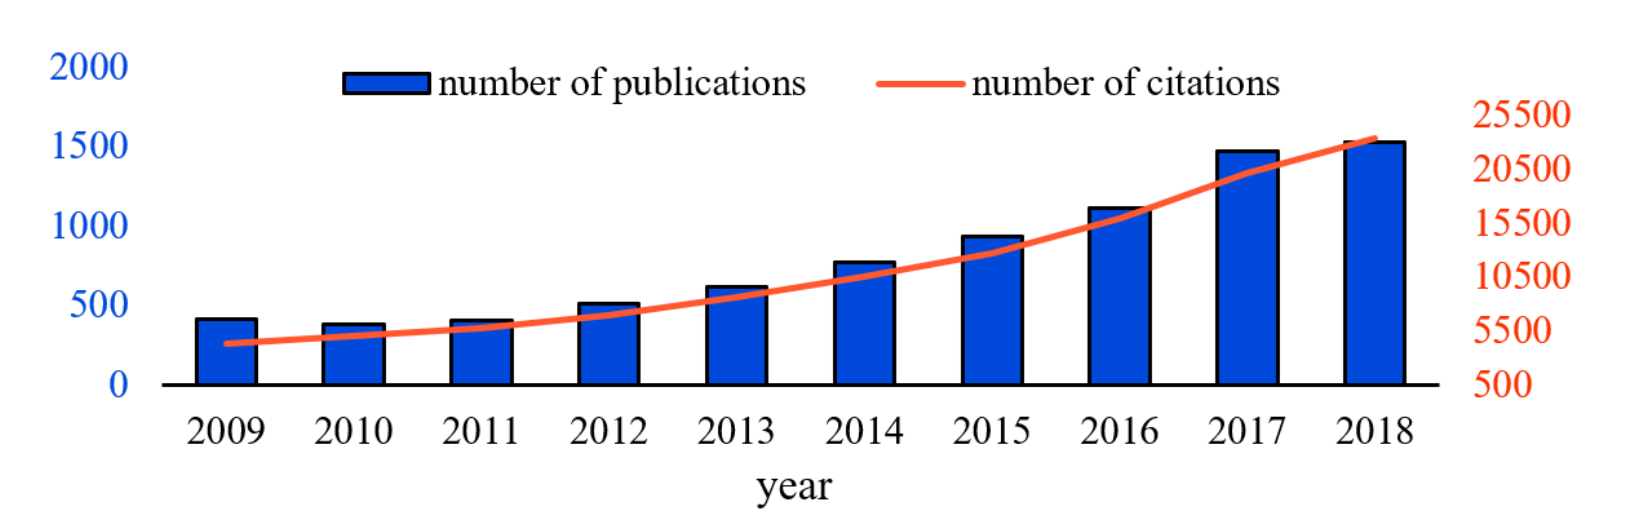
\includegraphics[width=0.5\textwidth]{img/cars_papers.png}
    \caption{Numbers of publications and citations in autonomous driving research over the past decade \cite{unknown}}
    \label{fig:cars_papers}
\end{figure}

\section{Application of swarm robotics}

As mentioned in the previous section, one of the properties which defines swarm systems is their great flexibility and this is reflected in the amount of fields in which swarm systems are recognized to be of great use. \\
Autonomous cars are highly considered the future of the car industry and this is shown in the fact that the number of papers about the topic is rapidly increasing as years go by, as shown in Fig. n. \ref{fig:cars_papers} \cite{unknown}.\\
\begin{figure}[htb]
    \centering
    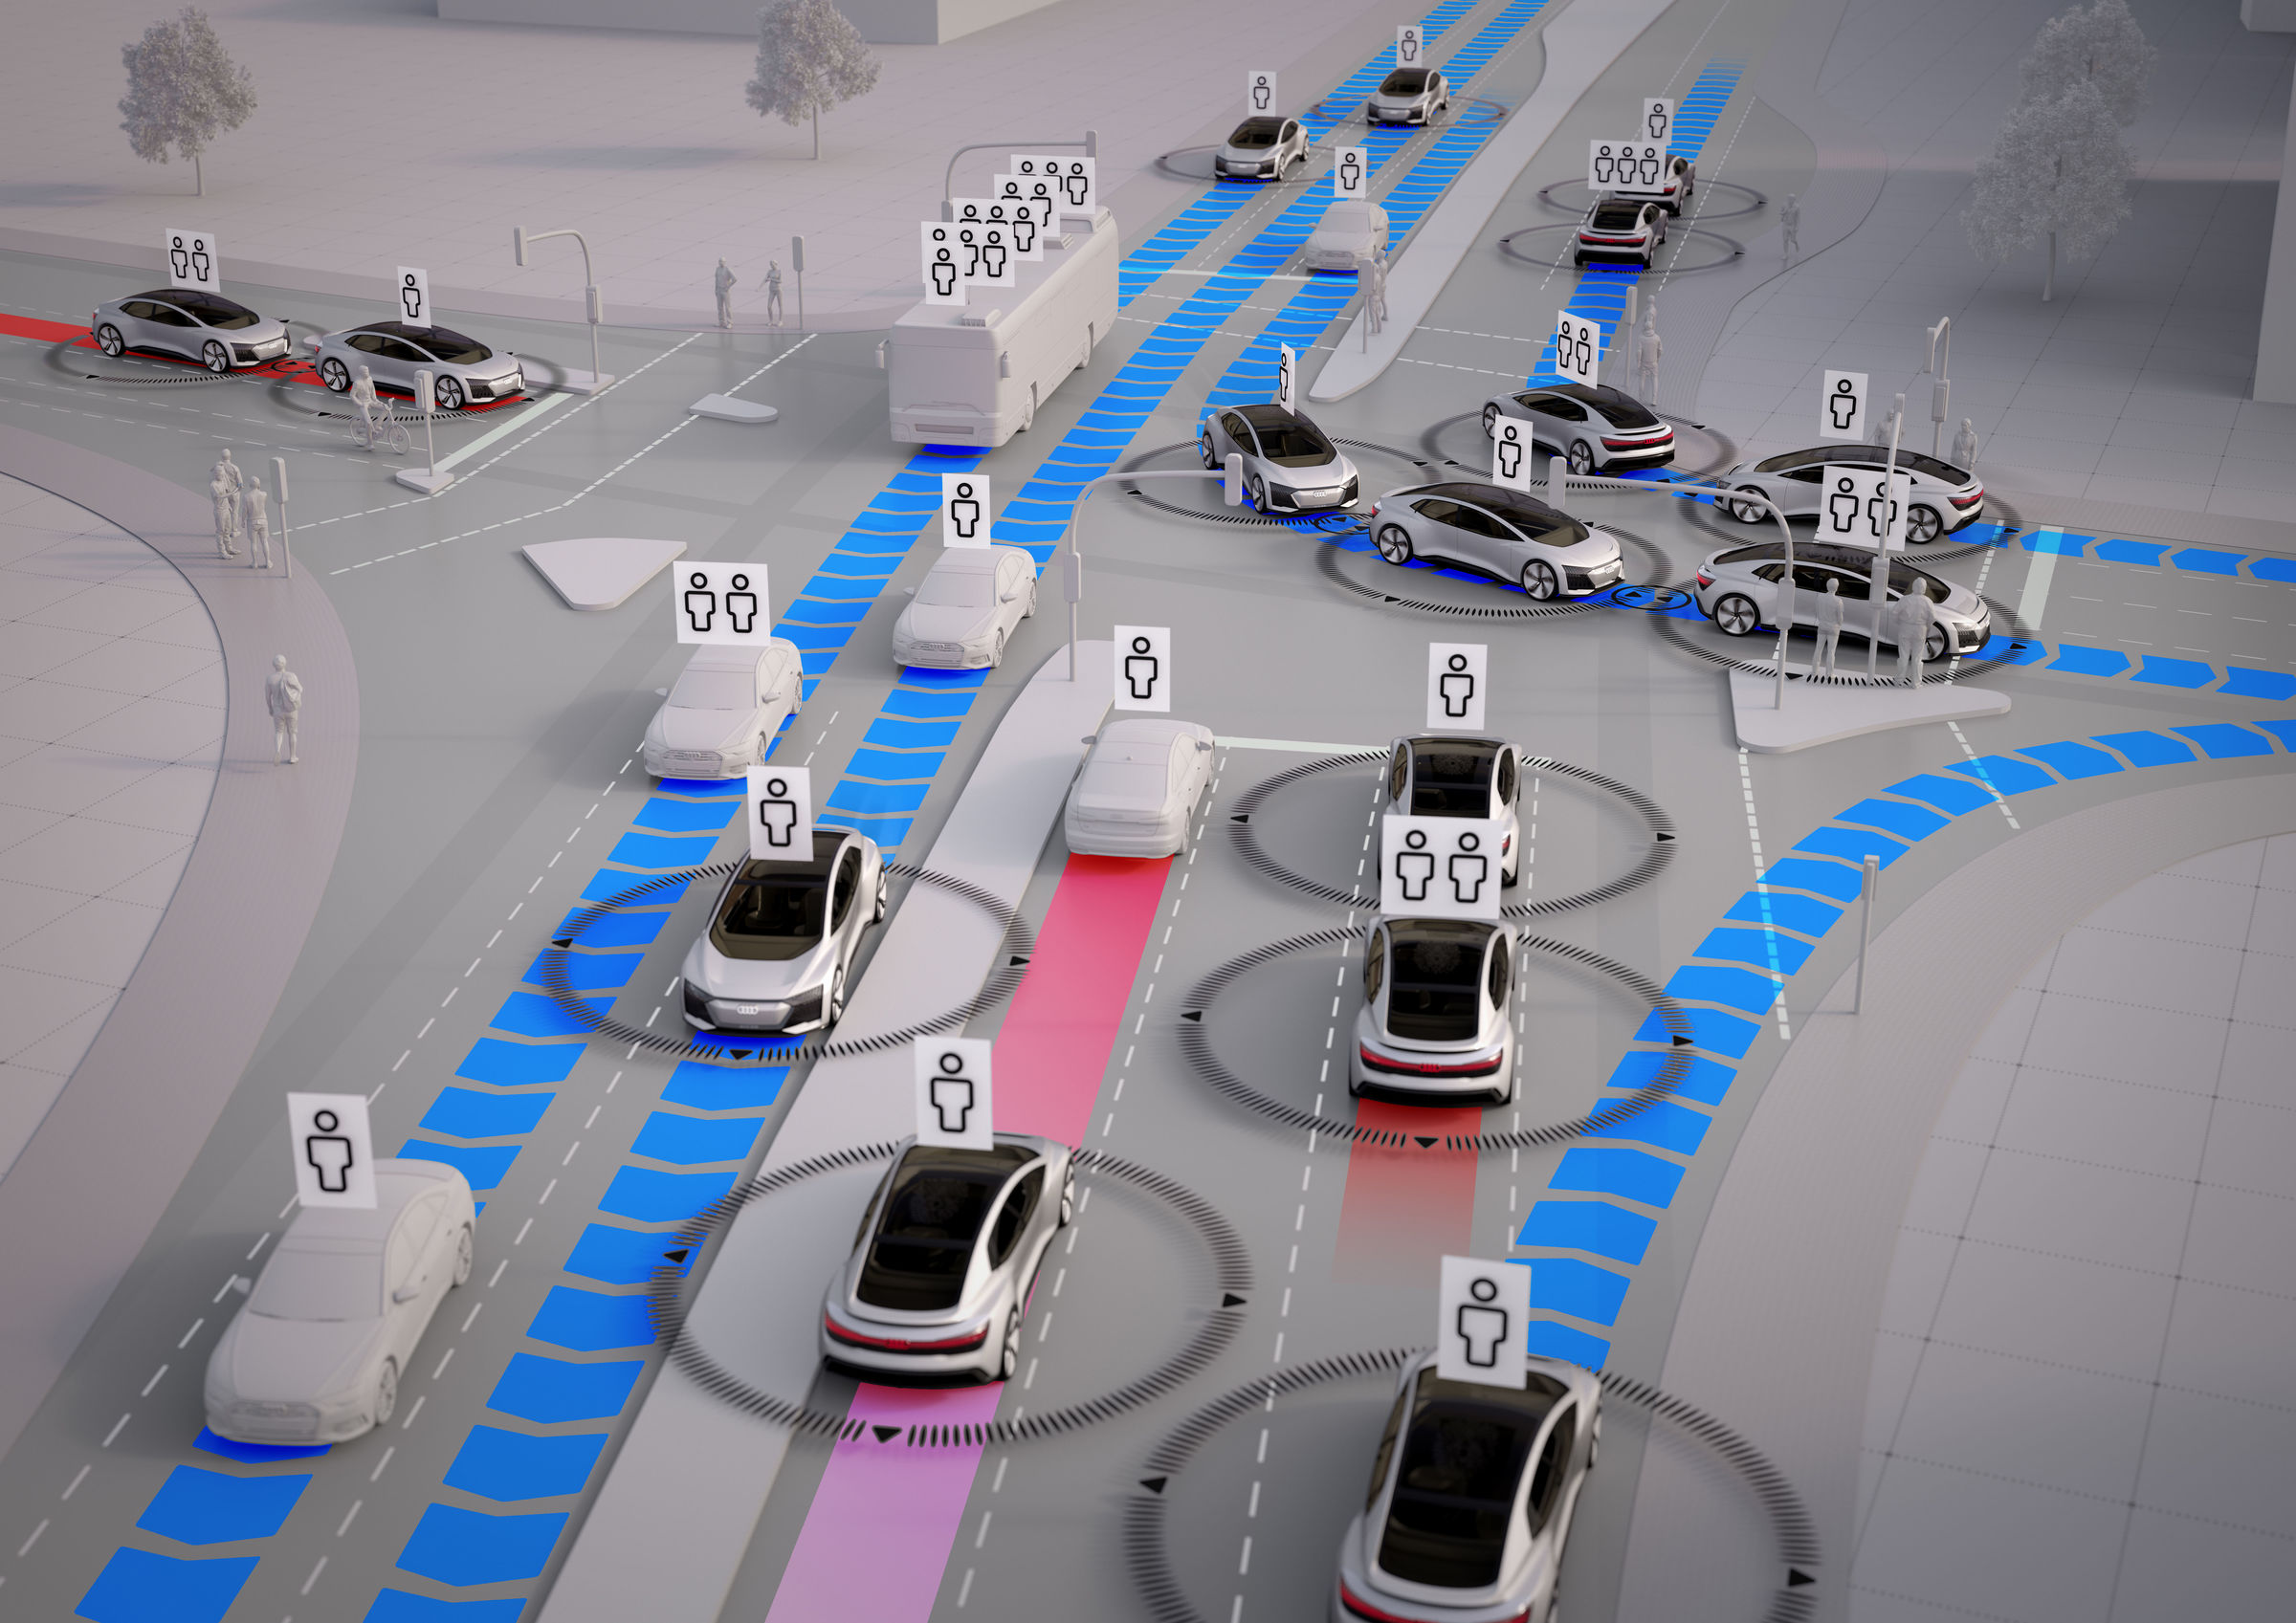
\includegraphics[width=0.5\textwidth]{img/future_city.jpg}
    \caption{Audi study "25th Hour – Flow": No Congestion in the City of the Future (Example City Ingolstadt) \cite{AUDI_CAR}}
    \label{fig:future_city}
\end{figure}
Although the technology is advancing at an unprecedentedly fast pace, so fast in fact that technologies become obsolete within years \cite{unknown}, many still questions the safety of this new way of conceiving road mobility (\cite{Johnson+2020+137+155}, \cite{robert_are_2019}). To increase safety for passengers in autonomous vehicles, German car manufacturers Audi and Daimler consider swarm robotics as the main solution. (\cite{AUDI_CAR}, \cite{daimler}).\\
Both visions share a particular term: "Car-to-X" principle. The Car-to-x principle can be thought as an augmentation of both the Vehicle-to-infrastructure (V2I) and the Vehicle-to-Vehicle (V2V) principles. Basically, according to this principle, every car exploits the properties of 5G to communicate not only with other cars, but also with every other entity in the environment to receive information about traffic, parking spots, various dangerous like icy roads or bikers, etc. (Fig n. \ref{fig:future_city}). 
The information are then dealt with using swarm intelligence techniques to achieve the most stable, flexible and robust system possible. \\
As Audi claims "The car-to-x technologies developed by Audi open up numerous new possibilities for making driving safer, more relaxed, and more intelligent"\cite{AUDI_CAR}. \\
Where swarm robotics technologies really shine, however, is in the farming field. According to some, farming is now undergoing a revolution thanks to swarm robotics. \cite{revolution}\\
One of the most notable example is the Swarm Robotics for Agricultural Applications (SAGA) project. \cite{Albani:2017tp} \cite{AlbaniEtAl:BICT2019}\\
The main goal of this project is to demonstrate the advantages of multi-robot systems, guided by swarm intelligence principles, working in farms over the current state of the art within the context of monitor/mapping. \cite{Albani:2017tp}\\
Unmanned Aerial Vehicles (UAVs) are programmed to work collectively in order to build a map of the field,in which the plantation is divided in different areas with different semantic tags in such a way that the spatio-temporal planning of weeding operations is facilitate, also with the use of autonomous precision weed removal robots.

\begin{figure}[htb]
    \centering
    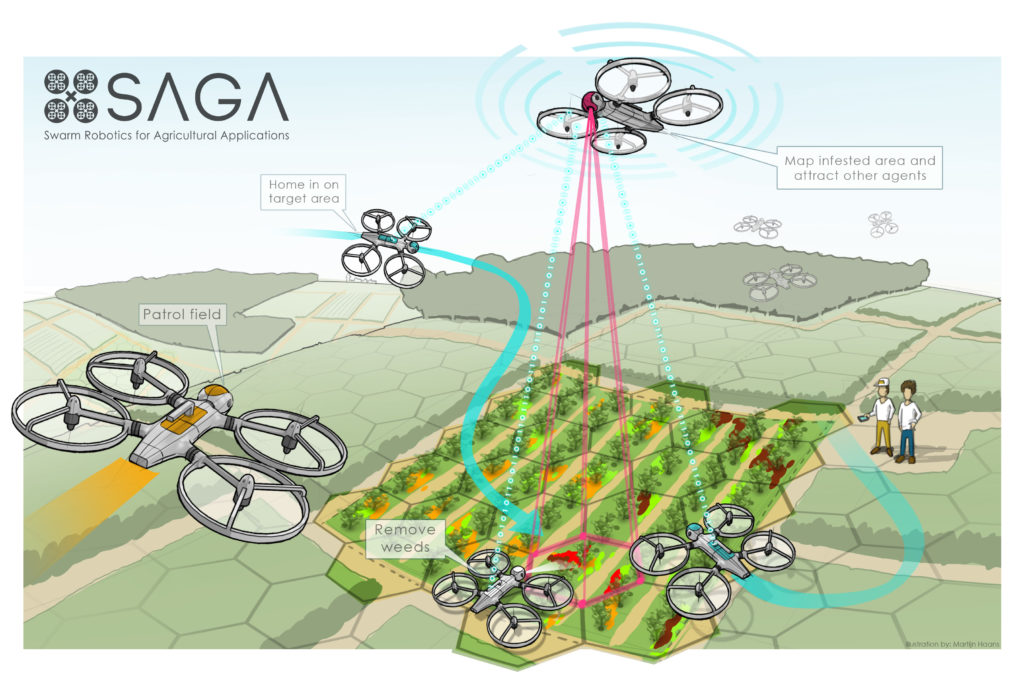
\includegraphics[width=0.5\textwidth]{img/saga.jpg}
    \caption{Vision of the Saga project (https://echord.eu/saga.html) }
    \label{fig:saga_project}
\end{figure}

The application of swarm robotics in Agriculture, however, is not limited to the monitor scenario or for inspection tasks, like the solution proposed by Carbone et al. in \cite{Carbone2018}, but rather applicable to every other scenario. As a matter of fact, Fichtl et al. in \cite{Fichtl2019FeldschwarmModularAS} proposes a concept consisting of tractors with an intelligent and modular (tillage) unit using swarm intelligence to cooperate with each other. 


\section{Deep Learning and Deep Reinforcement Learning}\label{Deep_learning_DRL}
Deep learning (DL) is a subset of the broader family of Machine Learning based mainly on Neural Networks (NN)  with representation learning, which is a set of techniques that allows a system to identify the characteristics needed for feature detection or classification from raw data. \\
As pointed out by LeCun et al. in \cite{deep_learning}, "Deep-learning methods are representation-learning\footnote{Representation learning is a set of methods that allows a machine to be fed with raw data and to automatically discover the representations needed for detection or classification \cite{deep_learning}} methods with multiple levels of representation, obtained by composing simple but non-linear modules that each transform the representation at one level into a representation at a higher, slightly more abstract level". 
Nowadays deep learning technologies are being applied in almost any field, from the medical one to autonomous cars. It is omnipresent, in every aspect of our lives and that is due to the incredible amount of doors that it can open. 
However, despite being very advantageous,deep learning has also been proven very challenging. 
As delineated by Razzak et al. in \cite{Razzak2018}, for example, deep learning techniques are expecting to bring significant improvements in the high priority sector like the healthcare one, however it is still facing problems that need to be solved. 
\begin{figure}[htb]
    \centering
    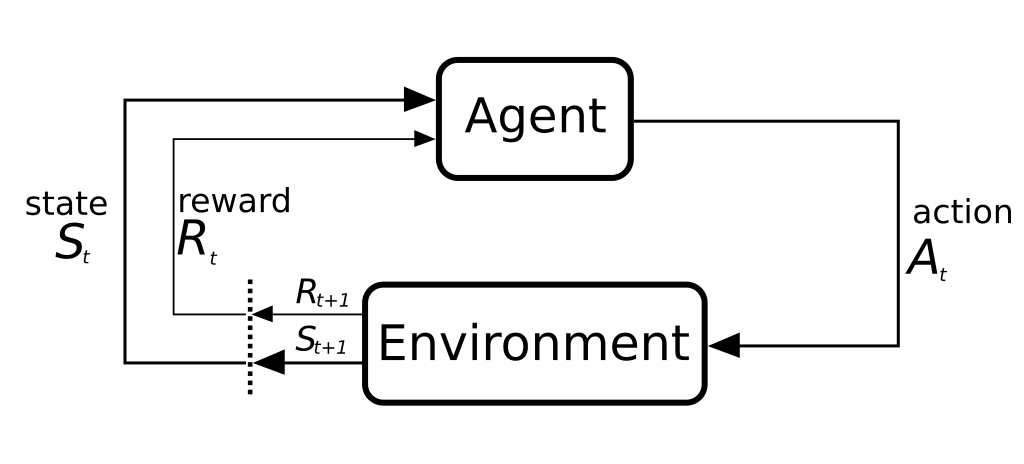
\includegraphics[width=0.5\textwidth]{img/markov_dia.png}
    \caption[Ciao]{Representation of the Markov diagram \cite{enwiki:1060247210}
    }
    \label{fig:m_dia}
\end{figure}


Deep Reinforcement Learning is a sub-field of machine learning with the main focus of combining reinforcement learning with deep learning. \\
Reinforcement learning is a process in which agents try to learn from the outcome of their decisions. This type of problems are often modeled mathematically as Markov decision processes. In very simplistic words, in such models, agents take an action $a$ when in a state $s$ receiving a reward before transitioning to the next state named $s'$. The purpose of the agents is to learn a policy $\pi(a|s)$ or map from observations to actions, in order to maximize its returns (expected sum of rewards)\cite{DBLP:journals/corr/Li17b}. An overview of such process can be seen in Fig n. \ref{fig:m_dia}. \\
An RL agent includes one or more of the following components:
\begin{itemize}
    \item  a representation of a \textit{value function} that provides a prediction of how good each action $a$ in a particular state $s$ is,
    \item a direct representation of the policy $\pi(s|a)$
\end{itemize}

In real world practical applications, the state space is high-dimensional and possibly continuous, and traditional reinforcement learning techniques might not suitable. The use of neural networks, however, allows those techniques to behave correctly since neural networks are well suited for dealing with high-dimensional sensory inputs and can be trained incrementally as well \cite{DBLP:journals/corr/Li17b}.



For the sake of this paper, we will focus on the simplest and most popular value-based algorithm, namely the Q-learning algorithm. \\
The Q-learning algorithm uses an off-policy method that separates the acting policy from the learning one and can be expressed by the following equation (\cite{Q_learning}):
\begin{equation}
    Q(s,a) \leftarrow Q(s,a) + \alpha [R + \gamma max( Q(s',a')) - Q(s,a)]
    \label{q_value}
\end{equation}
where:
\begin{enumerate}
    \item $\alpha$ is the learning rate with a value between 0 and 1
    \item $R$ is the reward, which is calculated by a so called reward function
    \item $Q(s,a)$ is the current Q value. This term is often referred as the old value.
    \item $Q(s',a')$ is the Q value given the next state and the action. It is worth pointing out that this value is an estimate of the optimal future value
    
\end{enumerate}

The Q-value $Q(s,a)$ is updated at every step given the sum of already existing q-values and the equation which determines the best action in the current state. Updating the Q-value using the aforementioned equation is referred to as Q-learning.\cite{Q_learning}\\
During the training process, a table usually called Q-table containing the rewards relative to the state-action pair is updated and it can be then queried to solve given problems. The Q-table can be initialized with either random values or to zero, like in Fig n. \ref{fig:q_table}
\begin{figure}[htb]
    \centering
    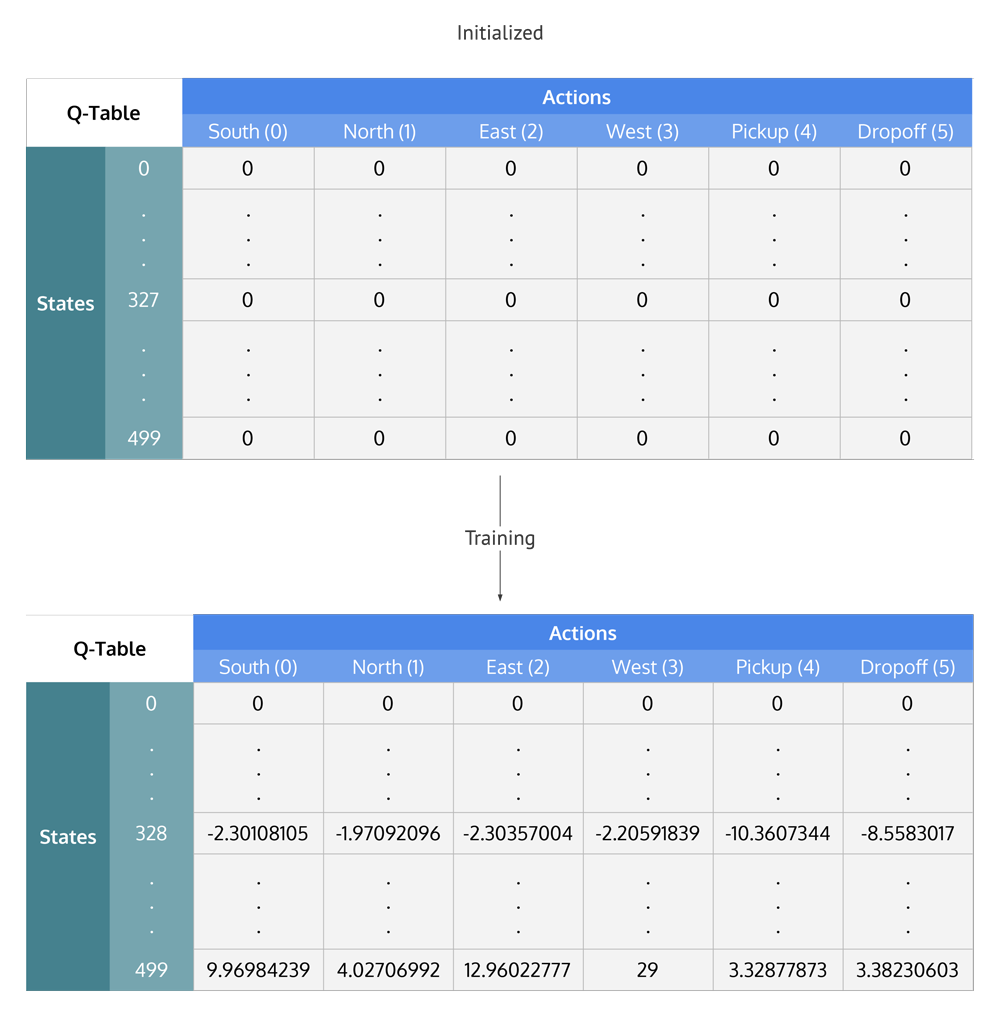
\includegraphics[width=0.4\textwidth]{img/Q-Learning_Matrix_Initialized_and_After_Training.png}
    \caption{Q-Learning table of states by actions that is initialized to zero, then each cell is updated through training\cite{enwiki:1054401845} 
    } 
    \label{fig:q_table}
\end{figure}

The Q-learning approach has become the basis of many reinforcement learning algorithms because of its simplicity and excellent learning ability in single-agent environments. \cite{Q_learning}\\
Although simple and elegant, this approach tends to be not very effective when solving problems in large or in multi-agent environments,like the real world, because the permutation state-action is so immense that some actions might not have been experienced previously. In addition, the number of cells in the Q-table grows exponentially with the number of action states, therefore requiring a considerably large amount of memory. \cite{Q_learning}\\
Deep Q-learning was developed by Google Deep Mind to obviate to the problem of memory in large environments. Deep Q-learning uses a Convolutional Neural Network as an approximation function when it becomes too difficult to express the value function for every state.
\cite{Q_learning}\\
Since the value approximation may result unstable if there is too much correlation with the training data, Deep Q-learning uses two strategies to reduce it, namely replay memory, or experience replay, and the so-called target Q technique. 
The experience replay approach uses a buffer, namely the replay memory, to store the experience, i.e. all the states, actions and rewards, which will then be queried randomly for a batch of data with arbitrary size, hence removing correlation all together. \cite{Q_learning}\\
The target Q technique, on the other hand, uses a separate neural network, the so called target network, to obtain the target value and train the Q network based on that target value, which helps reducing correlation. \cite{Q_learning}\\



\section{Deep  Learning in Swarm Driving}
As we pointed out in section 1, cooperation can augment the capabilities of a single individual. This concept can also be applied to robotics swarm, especially swarm based on resource-limited robots, to achieve results which otherwise could not be achieved. Usually, these systems tend to imitate biological processes. For example,  Kube et al in \cite{KUBE200085} modelled a scenario, based on the ants' behavior,  in which the robots have the goal of pushing a box. However, those scenarios become very complex to model the more they approach a real word application. To help flatten the difficulty, one solution is to use deep learning techniques. \\
The first application we are going to analyze is the one proposed by Hüttenrauch et al in \cite{guided}. In this paper, the authors simulate a swarm of agents based on the Kilobot (Fig n. \ref{fig:kilobot}), which is a very simple 3-legged robot with limitated sensing capabilites. 
The agents need to learn a specific policy by learning from their moves. 
They defined two policies: one to locate a target and one to build a graph with the other agents. To train the agents to solve these properties, the authors used an approach similar to the Deep Deterministic Policy Gradient Algorithm (DDPG). Hüttenrauch et al. concluded that this result \textit{"is not feasible with a non-guided approach"}. \cite{guided}\\
\begin{figure}[htb]
    \centering
    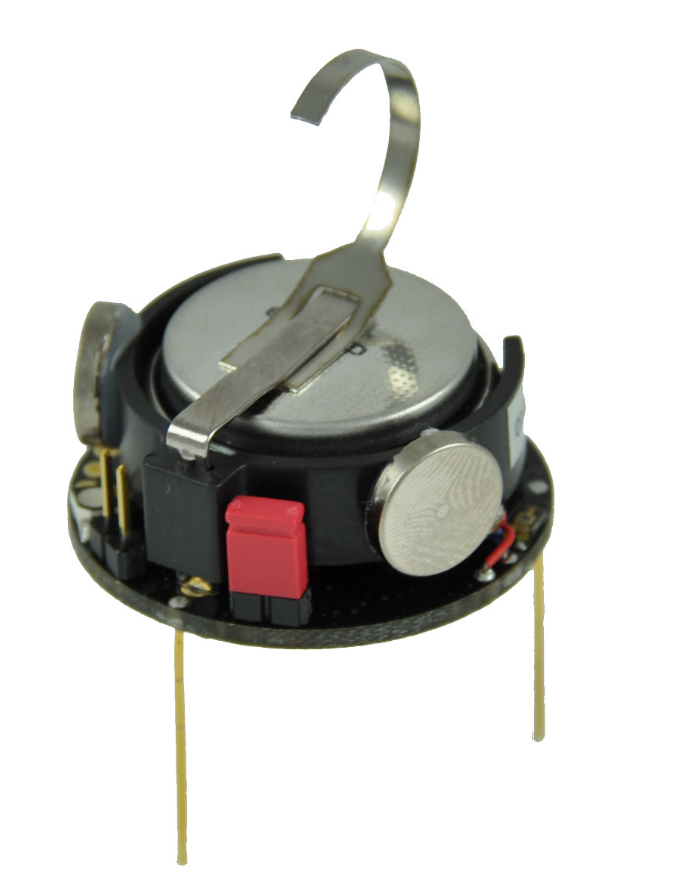
\includegraphics[width=0.3\textwidth]{img/Kilobot.png}
    \caption{The figure shows a Kilobot robot \cite{guided} }
    \label{fig:kilobot}
\end{figure}


A completely different approach is the one used by Nguyen et al. in \cite{nguyen2020continuous}. Similarly to what we observed previously, they also noticed that \textit{a swarm of multi-robot systems demands higher computational requirements as the swarm size increases}(\cite{nguyen2020continuous}), therefore posing a scalability problem. To overcome such problem the authors propose a solution inspired from the concept of shepherding. As a matter of fact, taking inspiration from sheep-dogs guiding a flock, they use a system comprised of one controlling agent, namely an unmanned areal vehicle (UAV), acting as a sheepdog which controls three unmanned ground vehicles (UGVs). The UAV has a global perspective of the environment, hence is able to communicate with the other UGVs and those are within the field of view of its camera, and its job is to guide them towards a target. \\
Differently from the solution proposed in \cite{guided}, which was a simulation in a controlled environment, Nguyen et al. could not model the behavior of the swarm using only a limited set of moves (backwards, forwards, left and right) since they are acting on a closer-to-real-world environment, where the action space of the robots is continuous.
To overcome this problem,  Nguyen et al. applied an Hierarchical Deep Deterministic Policy Gradient (H-DDPG) algorithm to the UGVs and a DDPG to the UAV.
The DDPG algorithm employs an architecture that comprises two networks, rather than only one, namely the agent and the critic. The first one, the agent network, estimates the policy as a continuous value, while the critic network simply approximates the Q-value corresponding to said policy. \\
This system has been tested both in a simulated and in a physical environment, with \textit{"near-optimal"} results. The authors concluded from this experiment that \textit{"the differences in performances between the simulation and the physical environment is insignificant"}\cite{nguyen2020continuous}. \\




\usetikzlibrary{decorations.pathreplacing}
\begin{figure*}[thb!]
	\centering
	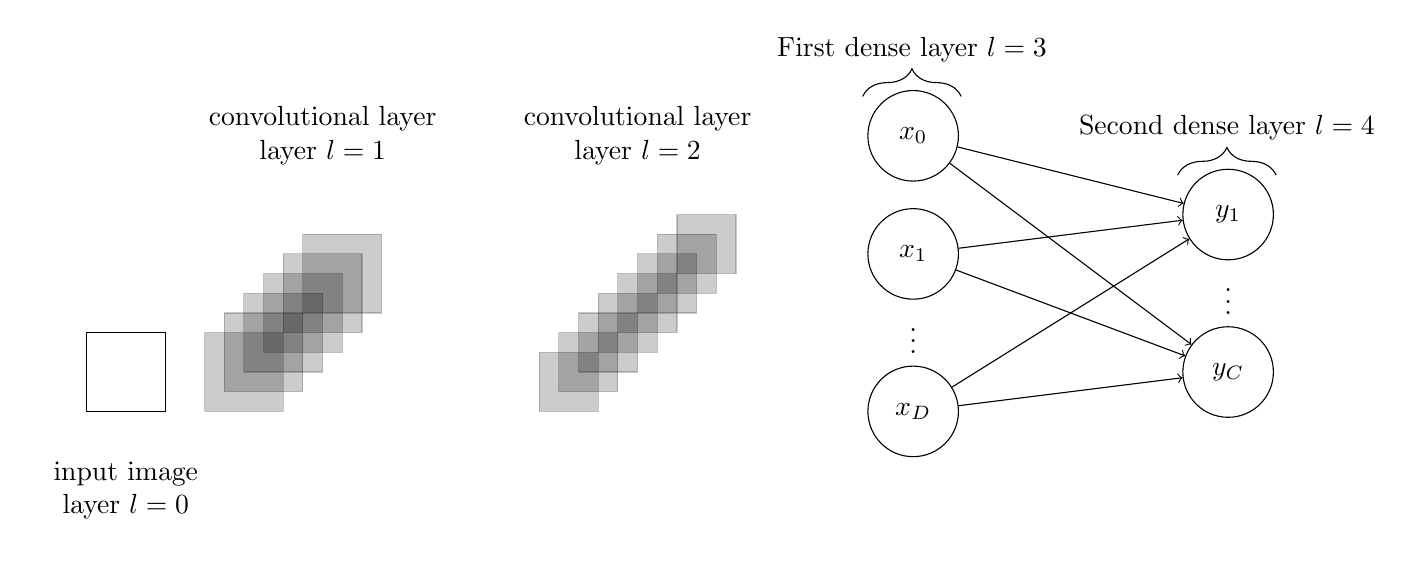
\begin{tikzpicture}
		\node at (0.5,-1){\begin{tabular}{c}input image\\layer $l = 0$\end{tabular}};
		
		\draw (0,0) -- (1,0) -- (1,1) -- (0,1) -- (0,0);
		
		\node at (3,3.5){\begin{tabular}{c}convolutional layer\\layer $l = 1$\end{tabular}};
		
		\draw[fill=black,opacity=0.2,draw=black] (2.75,1.25) -- (3.75,1.25) -- (3.75,2.25) -- (2.75,2.25) -- (2.75,1.25);
		\draw[fill=black,opacity=0.2,draw=black] (2.5,1) -- (3.5,1) -- (3.5,2) -- (2.5,2) -- (2.5,1);
		\draw[fill=black,opacity=0.2,draw=black] (2.25,0.75) -- (3.25,0.75) -- (3.25,1.75) -- (2.25,1.75) -- (2.25,0.75);
		\draw[fill=black,opacity=0.2,draw=black] (2,0.5) -- (3,0.5) -- (3,1.5) -- (2,1.5) -- (2,0.5);
		\draw[fill=black,opacity=0.2,draw=black] (1.75,0.25) -- (2.75,0.25) -- (2.75,1.25) -- (1.75,1.25) -- (1.75,0.25);
		\draw[fill=black,opacity=0.2,draw=black] (1.5,0) -- (2.5,0) -- (2.5,1) -- (1.5,1) -- (1.5,0);
		
		\node at (7,3.5){\begin{tabular}{c}convolutional layer\\layer $l = 2$\end{tabular}};
		
		\draw[fill=black,opacity=0.2,draw=black] (7.5,1.75) -- (8.25,1.75) -- (8.25,2.5) -- (7.5,2.5) -- (7.5,1.75);
		\draw[fill=black,opacity=0.2,draw=black] (7.25,1.5) -- (8,1.5) -- (8,2.25) -- (7.25,2.25) -- (7.25,1.5);
		\draw[fill=black,opacity=0.2,draw=black] (7,1.25) -- (7.75,1.25) -- (7.75,2) -- (7,2) -- (7,1.25);
		\draw[fill=black,opacity=0.2,draw=black] (6.75,1) -- (7.5,1) -- (7.5,1.75) -- (6.75,1.75) -- (6.75,1);
		\draw[fill=black,opacity=0.2,draw=black] (6.5,0.75) -- (7.25,0.75) -- (7.25,1.5) -- (6.5,1.5) -- (6.5,0.75);
		\draw[fill=black,opacity=0.2,draw=black] (6.25,0.5) -- (7,0.5) -- (7,1.25) -- (6.25,1.25) -- (6.25,0.5);
		\draw[fill=black,opacity=0.2,draw=black] (6,0.25) -- (6.75,0.25) -- (6.75,1) -- (6,1) -- (6,0.25);
		\draw[fill=black,opacity=0.2,draw=black] (5.75,0) -- (6.5,0) -- (6.5,0.75) -- (5.75,0.75) -- (5.75,0);


		\tikzstyle{unit}=[draw,shape=circle,minimum size=1.15cm]
 
        \node[unit](x0) at (10.5,3.5){$x_0$};
        \node[unit](x1) at (10.5,2){$x_1$};
        \node(dots) at (10.5,1){\vdots};
        \node[unit](xd) at (10.5,0){$x_D$};
 
        \node[unit](y1) at (14.5,2.5){$y_1$};
        \node(dots) at (14.5,1.5){\vdots};
        \node[unit](yc) at (14.5,0.5){$y_C$};
 
        \draw[->] (x0) -- (y1);
        \draw[->] (x0) -- (yc);
 
        \draw[->] (x1) -- (y1);
        \draw[->] (x1) -- (yc);
 
        \draw[->] (xd) -- (y1);
        \draw[->] (xd) -- (yc);
 
        \draw [decorate,decoration={brace,amplitude=10pt},xshift=-4pt,yshift=0pt] (10,4) -- (11.25,4) node [black,midway,yshift=+0.6cm]{First dense layer $l = 3$};
        \draw [decorate,decoration={brace,amplitude=10pt},xshift=-4pt,yshift=0pt] (14,3) -- (15.25,3) node [black,midway,yshift=+0.6cm]{Second dense layer $l = 4$};
	\end{tikzpicture}
\caption{ Architecture of the convolutional neural network used in the use case. Layer $l=0$ is the input layer, with dimension $10 \times10\times 3$, hence a 10 by 10 RGB image (3 channels); $l= 1$ is the first convolution layer with a kernel of $3\times3$ and an input shape of $10 \times10\times 3$; $l=2$ is the second convolution layer with a kernel of $3\times 3$;$l=3$ is the first dense layer with an input size of $64$ and an output size of $32$;$l=4$ is the final dense layer, with an input size of $32$ and an output size of $9$ }
	\label{fig:example-convolutional-network}
\end{figure*}


%\section{others }
%\cite{deseases}
%\cite{7553030a}
%\cite{2020}


%\section{Problems in communication }
%\cite{9040539}
\section{Use Case}
Using what we learned in the previous sections we are now able to analyze an use case of a Deep-Q-learning algorithm use to train agents towards a specific goal. \\
The goal of our agents in the simulation will be to create a swarm containing all the other robots scattered in the field.
The creation of a swarm requires that all the robots are within a set distance from each other and, with this distance, we are simulating the possible communication range of each robots. We imagined those robots not to be particularly powerful, hence it is safe to assume that they would have a limited communication range.\\
The swarm we want to build is modelled using a graph, hence the goal of the agents is to establish a graph with the nodes being the agents and the edges being the distance between them (which should be less than an arbitrary value, i.e. the communication range). We expect the agents to have a global understanding of environment, hence they know the position of all the others.\\
To further simplify the simulation, we are assuming to operate in a discrete environment, hence  we expect the robots to possibly make only 9 discrete moves, defined as:
\[
    up,left, rigth,down, up-left,
\]
\[
    up-right, down-left, down-right
\]
The robot can move of one unit in one of the above mentioned directions in a 10x10 units large environment.\\
In this simulation, we will use a Deep-Q-learning model to predict the Q-value and learn a policy defined by a rather simple reward function. The reward function gives high rewards if the agent is moving towards the already established graph, if it creates a new one or if it becomes part of an already existing one. The highest value amongst those is given if the agent enters in the graph and it completes it. The lowest value, on the other hand, is given if the robot is moving further away from the graph or if it exits the graph. Furthermore, the agents are penalized if they take too many steps before completing the graph sine we would like the robots to create the swarm efficiently.\\ 
The network used is a simple Convolutional Neural Network (CNN) which is fed with an image representing the environment and predicts the next Q-value accordingly. A representation of the model can be found in Fig. n. \ref{fig:example-convolutional-network}. \\
As we discussed in Section \ref{Deep_learning_DRL}, to make the network more stable we also use a target network and a replay memory. \\
The training for the model is carried out by 5000 episodes and 3 agents and the starting position is determined randomly at the beginning of each episode. The validation is carried out similarly, with a lower number of episodes, namely 100, with a different seed for the random number generator. The results are promising, with an accuracy of 100\%, meaning that the agents are able to create a swarm each time. This is due to the fact that the environment is limited and discrete, hence not too difficult to learn.
As we discussed in \ref{sec:swarm}, swarm robotics applications need to respect certain criteria,namely  scalability and robustness.  \\
In order to check both scalabilty, we can increment both the number of agents and the dimensions of the environment. In other words, using the models we trained before, we can train them to work in a 15x15 space with a new agent as well. With just 100 epochs for training, the agents are able to create a swarm 95\% of the times in our 100 epochs validation test. \\
To check the robustness of the models, we can add an area in the environment over which the robots can not fly. In this way we can simulate a dangerous area over which the robots can not fly. It could be a wall, a physical obstacle in general or even an area that could not be identified in case there is an other device that is providing the global status to the robots. \\
We also need to slightly changing the reward function. The highest punishment is now assigned in case the robots are moving in this area or towards it. On the other hand, if the robots move further away, they get rewarded with a high value. The first training cycle with 100 episodes showed an interesting behavior. During this training cycle, the robots were only punished if moving towards the area and the model reached an accuracy only 4\%. The agents did not learn to move around the obstacle, on the other hand, they tried to create the graphs anyway because the rewards was higher. When the rewards was added once again, the drones learned around the 50th episode to circumnavigate the obstacle and to stay as far away as possible from it. In addition, we could see a change in strategy. In fact, if before the introduction of the obstacle the agents tried to ''meet'' in the upper part of the field, now they are trying to meet in the part of the field which is both bigger and further away from the obstacle. 
With a training lasting other 100 episodes, the accuracy raised to 49\%, an increment of 45\% compared to the previous cycle, but still far from the 95\% achieved without the obstacle. However, the last  value has been achieved with a training cycle of 5000 episodes, while the last value has been achieved with only 200. \\
From these results we can prove not only that the system we developed is in fact robust, but also that is able to adapt to new conditions in the environment. 
\section{Conclusion}
Swarm driving is a relatively new field which has raised a lot of attention recently in both academia and industry. Swarms allow more stable, safer and more secure systems, with a lower use of resources and money. As a matter of fact, swarm driving is being applied to fields like autonomous driving and smart farming, which are historically expensive and high-performance demanding.  
However, the complexity of these systems can reach very high levels in real world scenarios and therefore making their actual deployment and development impossible due to physical resource constraints. 
In this paper, we analyzed the vast field of swarm robotics, describing the many advancements it can bring, the fields which would mostly benefit and the challenges that still need to be faced. We explored how some of these challenges can be solved using Deep Learning by studying some innovative solutions that are achieving promising results. In addition, we have been able to develop a simulation of a swarm driven by Deep Q Learning and we manage to build a flexible, scalable and robust system. \\
Although these solutions are still on a primitive stage and there are still many challenges to tackle, the results obtained are remarkable and prospect a very bright future for this field, which could change what we deem as possible and impossible.\\

%\cite{guided}


%\cite{deep_learning}
\newpage

\bibliographystyle{ieeetr}
\bibliography{mybibfile}



\end{document}
